\section{Classification of covariance matrices}
\label{sec:classofcov}


\subsection{Fundamentals of classification}
\label{subsec:fund_class}

\iflatexml\else \changes{ \fi
Given labelled samples $\x_i$ drawn from two classes or populations (positive and negative), a simple classification algorithm consists in assigning a previously unseen sample to the class with closer mean.
This implies a computation of means of class and a measure of distances from the means. 
Assuming that the samples are embedded into a dot product space (i.e. with Euclidean geometry), the means can be computed as:
\iflatexml\else } \fi

\begin{equation}
c_{+} = \frac{1}{m_{+}} \sum_{ \left\lbrace i|y_i=+1 \right\rbrace } \x_i,
\label{eq:mean_eucl1}
\end{equation}

\begin{equation}
c_{-} = \frac{1}{m_{-}} \sum_{ \left\lbrace i|y_i=-1 \right\rbrace } \x_i,
\label{eq:mean_eucl2}
\end{equation}
\iflatexml\else \changes{ \fi
where $y_i \in \left\lbrace +1, -1 \right\rbrace$ is the label of the training sample $\x_i$, $m_{+}$ and $m_{-}$ the number of positive and negative samples respectively. 
An unseen sample $\x$ is assigned to the class whose mean is the closest. 
This simple geometric classification framework is the founding principle of more complex algorithms such as supporting vector machines. 
\iflatexml\else } \fi

\iflatexml\else \changes{ \fi
It can be formulated in terms of the dot product $\left\langle \cdot, \cdot \right\rangle$.
If $c:=(c_{+}+c_{-})/2$ is the point lying halfway between $c_{+}$ and $c_{-}$, and $w:=c_{+}-c_{-}$ the vector connecting $c_{+}$ to $c_{-}$, the class label $y$ of the unseen sample $\x$ is determined by checking whether the vector $\x-c$ connecting $c$ to $x$ makes an angle $\alpha < \pi/2$ with $w$ [ref: fig].   
This is expressed as:
\iflatexml\else } \fi

\begin{equation}
\begin{split}
y &= \mathrm{sgn} \left\langle (\x-c),w \right\rangle \\
  &= \mathrm{sgn} \left\langle (\x-(c_{+}+c_{-})/2),(c_{+}-c_{-}) \right\rangle \\
  &= \mathrm{sgn} (\left\langle \x,c_{+} \right\rangle - \left\langle \x,c_{-} \right\rangle + b)
\end{split}
\label{eq:classif1}
\end{equation}
\iflatexml\else \changes{ \fi
where $\mathrm{sgn}$ is the sign function.
The offset $b$ vanishes if class means are equidistant to the origin \cite{scholkopf_learning_2001}.
Inserting \eqref{eq:mean_eucl1} and \eqref{eq:mean_eucl2} in \eqref{eq:classif1} yields:
\iflatexml\else } \fi

\begin{equation}
y = \mathrm{sgn} \left( \frac{1}{m_{+}} \sum_{ \left\lbrace i|y_i=+1 \right\rbrace } \left\langle \x,x_i \right\rangle - \frac{1}{m_{-}} \sum_{ \left\lbrace i|y_i=-1 \right\rbrace } \left\langle \x,\x_i \right\rangle + b \right) .
\label{eq:classif2}
\end{equation}

\iflatexml\else \changes{ \fi
Classifier \eqref{eq:classif2} can be generalized as:
\iflatexml\else } \fi

\begin{equation}
y = \mathrm{sgn} \left( \sum_{i=1}^{m} y_i \alpha_i \dist(\x,\x_i) + b \right) ,
\label{eq:classif_gen}
\end{equation}
\iflatexml\else \changes{ \fi
where $\alpha_i$ is the weight of the training sample $x_i$ and $\dist(\cdot, \cdot)$ a distance, a divergence of a kernel. 
In the case of two classes, with $m$ samples ($m = m_{+} + m_{-}$) in the dot product space where all samples have the same weight, $y_i \in \left\lbrace +1, -1 \right\rbrace$, $\alpha_i = 1/m$ and $\dist(\cdot, \cdot) = \left\langle \cdot, \cdot \right\rangle$. 
\iflatexml\else } \fi

\iflatexml\else \changes{ \fi
Expression~\eqref{eq:classif_gen} corresponds to the decision function used in hyperplane classifiers \cite{scholkopf_learning_2001}. 
This shows that even more complex classifiers rely on the calculations of class means (or centers) and their distances to individual samples.
This being shown, in this article we focus on the simple classification approach of assigning a previously unseen sample to the class with closest mean.
\iflatexml\else } \fi

\iflatexml\else \changes{ \fi
In machine learning algorithms, samples are represented by their features which are determined through a feature extraction and selection process.
In this work, samples are represented by their covariance matrices. Therefore means of classes and distances to mean will be means of covariance matrices and distance between them.
\iflatexml\else } \fi

\subsection{Means of covariance matrices}
\label{subsec:mean}

\iflatexml\else \changes{ \fi
Consider a multivariate variable $\X \in \Re^{\dc \times \dt}$ where $\dc$ is the number of variables and $\dt$ the number of samples, with $C > N $, the covariance matrix of the centered variable $\X$ can be estimated as:
\iflatexml\else } \fi

\begin{equation}
\P = \frac{1}{\dt} \X \X^\intercal
\end{equation}
\iflatexml\else \changes{ \fi
and is symmetric positive definite (SPD): $\P \in \Ma$, a manifold of $\dc\times\dc$ symmetric positive definite matrices,
\iflatexml\else } \fi
\begin{equation*}
	\label{eq:rm}
  \Ma = \left\{ \P \in  \Re^{\dc\times\dc} : \P = \P^\intercal \text{ and } x^\intercal \P x > 0, \forall x \in \Re^{\dc} \backslash 0 \right\} \ . %\nonumber
\end{equation*}
The properties of SPD matrices constrain them to a convex cone:

\begin{enumerate}
[label=(\roman*)]
\item Symmetry: \tab $\P = \P^\intercal$ ,
\item Positive definiteness: \tab $\x^\intercal \P \x > 0, \forall x \in \Re^{\dc} \backslash 0$ ,
\item Strict positivity of diagonal element: \tab $\P(i,j) > 0 | i=j, \forall i,j \in \left\lbrace 1, \dots, \dc \right\rbrace$ i.e. positive variance ,
\item Cauchy-Schwarz inequalities: \tab $|\P(i,j)| \leq (\P(i,i) \P(j,j))^{1/2}, \forall i,j \in \left\lbrace 1, \dots, \dc \right\rbrace$ .
\end{enumerate}


\iflatexml\else \changes{ \fi
The mean of SPD matrices can be computed as a center of mass modeled on Euclidean geometry:
given a set of covariance matrices $\{\P_\nb\}_{\nb=1,\dots,\Nb}$,
the center of mass $\Pm$ of the set, is a covariance matrix that minimizes the sum of the squared distances to matrices $\P_\nb$:
\iflatexml\else } \fi

\begin{equation}
	\label{eq:mean}
	\Pm = \Rm(\P_1, \dots, \P_\Nb) = \argmin_{\P \in \Ma} \sum_{\nb=1}^{\Nb} \dist^2(\P_\nb,\P) \ ,
\end{equation}
where $\dist(\cdot,\cdot)$ is a measure of distance between two matrices. 
\iflatexml\else \changes{ \fi
Practically, $\dist(\cdot,\cdot)$ can either be a distance or a divergence.
\iflatexml\else } \fi

\iflatexml\else \changes{ \fi
In the literature, this  mean is at times designated as the \emph{Frechet mean}, \emph{Cartan mean}, or \emph{Karcher mean} \footnote{This appellation has been recently criticized by Karcher himself \cite{karcher_riemannian_2014}} \cite{ando2004geometric,lim_matrix_2012}.
Cartan \cite{cartan_groupes_1929} had shown that a unique solution to \eqref{eq:mean} exists if all $\P_\nb$ lie in a convex ball \citep[section 16 of][]{cartan_groupes_1929}. This applies also to closed convex cones.
\iflatexml\else } \fi

\iflatexml\else \changes{ \fi
Depending on the divergence or distance used, several means can be defined from \eqref{eq:mean}. Those considered in this study are presented in the next lines and summarized in Table~\ref{tab:dist}.
\iflatexml\else } \fi


\subsection{Distances and divergences}
\label{sec:distdiv}
\iflatexml\else \changes{ \fi
Divergences and distances are measures of dissimilarity between two points in a space.
Here a Riemannian space $\GenMa$ will be considered.
A distance function $\dist:\GenMa \times \GenMa \rightarrow \Re^+$ has the following properties for all $\P_1, \P_2,\P_3 \in \GenMa$:
\iflatexml\else } \fi

\begin{enumerate}
[label=(\roman*)]
\item Non-negativity: \tab $\dist(\P_1, \P_2) \geq 0$ ,
\item Identity: \tab $\dist(\P_1, \P_2) = 0 \ \ \mathrm{iff} \ \ \P_1 = \P_2$ ,
\item Symmetry: \tab $\dist(\P_1, \P_2) = \dist(\P_2, \P_1)$ ,
\item Triangular inequality:  \tab $\dist(\P_1, \P_3) \leq \dist(\P_1, \P_2) + \dist(\P_2, \P_3)$ .
\end{enumerate}
\iflatexml\else \changes{ \fi
Divergences are very similar to distances with the difference that properties (iii) and (iv) do not have to be satisfied. 
In the context of covariance matrices, divergences and distances should both induce a Riemannian metric on the manifold of SPD matrices. 
\iflatexml\else } \fi

\subsubsection{Euclidean distance}
\iflatexml\else \changes{ \fi
The Euclidean distance between two matrices is represented by the \emph{Frobenius norm} of their difference:
\iflatexml\else } \fi

\begin{equation}
\distF(\P_1, \P_2) = \lVert \P_1-\P_2 \rVert _F
\label{eq:dist_eucl}
\end{equation}
In \eqref{eq:mean}, this yields the arithmetic mean:

\begin{equation}
\PmE = \frac{1}{\Nb} \sum_{\nb=1}^{\Nb} \P_\nb
\label{eq:mean_arithmetic}
\end{equation}
The arithmetic mean is drawn from a family of power means ($\P_{t|t = 1}$)~\cite{lim_matrix_2012}:

\begin{equation}
\P_t = \left( \frac{1}{\Nb} \sum_{\nb=1}^{\Nb} \P_\nb^t \right)^{\frac{1}{t}}, \ t \in [-1,+1].
\label{eq:mean_power}
\end{equation}
\iflatexml\else \changes{ \fi
From the same family can be drawn the \emph{geometric mean} ($\P_{t|t \rightarrow 0}$) and the \emph{harmonic mean} ($\P_{t|t = -1}$).
\iflatexml\else } \fi

\iflatexml\else \changes{ \fi
We consider the arithmetic mean $\PmE$, as a baseline. 
This averaging of covariance is usually not adequate in the space of SPD matrices for two main reasons. 
Firstly, the Euclidean distance and averaging do not guarantee invariance under inversion: a matrix and its inverse are supposed to be at the same distance from the identity matrix. 
Secondly, the Euclidean averaging of covariance SPD leads to a \emph{swelling effect}: the determinant of the arithmetic mean of SPD matrices can be larger than the determinant of its individual components.
And since the determinant of a covariance matrix is a direct measure of the dispersion of the multivariate variable, the swelling effect introduces a large distortion of the data dispersion \cite{arsigny_geometric_2007}.
For these reasons, other means that adapt to the geometry of convex cone of SPD matrices are used. 
\iflatexml\else } \fi

\subsubsection{Affine Invariant Riemannian distance}
\iflatexml\else \changes{ \fi
The affine invariant Riemannian distance between two points is defined by the length of the curve connecting these point on the Riemannian manifold. 
A differential manifold is a topological curved space that is locally similar to the Euclidean space and is globally differentiable. 
The convex cone of SPD matrices is a manifold that can be endowed with a Riemannian metric; such manifolds are called Riemannian manifold.
Let $\GenMa$ be a Riemannian manifold, and $T_\P\GenMa$ its tangent space defined on point $\P$. 
A Riemannian metric $\metric$ is a family of inner product defined on the tangent spaces defined on each point $\P$ of the manifold.
This inner product varies smoothly from point to point on the manifold,
\[
 \metric_\P: T_\P\GenMa\times T_\P\GenMa \rightarrow \Re \]
$\metric$ is a function that assigns, for each point $\P \in \GenMa$, an inner product in the tangent space $T_\P\GenMa$  .
The Riemannian metric allows us to compute the length of vectors or distance between two point on the tangent space, and through appropriate mapping \cite{pennec_riemannian_2006}, the length of the corresponding \emph{geodesic} (i.e. the shortest curve connecting two point) on the manifold $\GenMa$.
The \emph{affine-invariant Riemannian distance} is the distance between two points of a Riemannian  manifold endowed with an invariant Riemannian metric $g_{\P}$ defined at $\P$:
\iflatexml\else } \fi
\begin{equation}
\begin{split}
g_{\P}(\S_1, \S_2) & = \left\langle \S_1 , \S_2 \right\rangle_\P \\
 & = \left\langle  \P^{-\frac{1}{2}} \S_1  \P^{-\frac{1}{2}} ,  \P^{-\frac{1}{2}} \S_2  \P^{-\frac{1}{2}} \right\rangle_\eye\\
 & = \tr \left( \P^{-\frac{1}{2}} \S_1 \P^{-1} \S_2 \P^{-\frac{1}{2}} \right) ,
\end{split}
\label{eq:metric-riemann}
\end{equation}
where $\eye$ is the identity matrix and $\tr$ the trace operator. 
The inner product of the tangent vectors $\S_1$ and $\S_2$ at $\P$ is invariant by the action of $\P^{-\frac{1}{2}}$ transformation.
The affine-invariant Riemannian distance is defined as:
\begin{equation}
\distAIRM(\P_1, \P_2) = \lVert \Log(\P_1^{-1}\P_2) \rVert_F = \left( \sum_{\chI=1}^{\dc} \log^2 \lambda_\chI \right)^{1/2},
\label{eq:dist_air}
\end{equation}
\iflatexml\else \changes{ \fi
where $\Log$ is the matrix logarithm instead of $\log$ for scalars, and $\lambda_\chI$, $\chI = 1, \dots, \dc$ are the eigenvalues of $\P_1^{-1}\P_2$.
\iflatexml\else } \fi

\iflatexml\else \changes{ \fi
Inserting \eqref{eq:dist_air} in \eqref{eq:mean} yields the mean $\PmAIRM$ associated to the affine-invariant Riemannian metric. 
It is the solution to 
\iflatexml\else } \fi
\begin{equation}
\sum_{\nb=1}^\Nb \Log(\PmAIRM^{-1/2} \P_\nb \PmAIRM^{-1/2})=0
\label{mean_air}
\end{equation}
It has no close form solution and can be solved iteratively through a gradient descent algorithm \cite{fletcher2004principal}. 

\iflatexml\else \changes{ \fi
These distance and mean are invariant to affine transformations. 
Some of these invariances are particularly important to preserve the geometric topology of the Riemannian manifold of SDP matrices. Let $f$ be an affine-invariant Riemannian function defined on $\GenMa$ (e.g. distance or mean),
\iflatexml\else }  \fi
\begin{enumerate}[label=(\roman*)]
\item \emph{Invariance under congruent transformation}
\begin{equation}
f(\P_1, \P_2) = f(\P \P_1 \P^\intercal, \P \P_2 \P^\intercal)
\label{eq:invar_congr}
\end{equation}
\item \emph{Invariance under inversion}
\begin{equation}
f(\P,\eye) = f(\P^{-1},\eye)
\label{eq:invar_invers}
\end{equation}
implying
\begin{equation}
f(\P_1,\P_2) = f(\P_1^{-1},\P_2^{-1})
\label{eq:invar_invers2}
\end{equation}
\end{enumerate}
Another interesting property of the affine-invariant Riemannian metric is its invariance to left- and right-multiplication by a positive matrix.
\begin{equation}
f(\P_1, \P_2) = f(\P \P_1, \P \P_2) = f(\P_1 \P, \P_2 \P)
\label{eq:invar_mult}
\end{equation}

\subsubsection{Log-Euclidean}
\iflatexml\else \changes{ \fi
The Log-Euclidean is another distance that takes into consideration the topology of Riemannian manifolds. 
It was introduced by Arsigny \textit{et al.} \citep{arsigny_geometric_2007} to alleviate the complexity involved in the computation of the affine-invariant Riemannian distance and its related mean.
The mean associated to the Log-Euclidean distance corresponds to an arithmetic mean in the domain of matrix algorithm.  
The distance between two SPD matrices is expressed as
\iflatexml\else } \fi
\begin{equation}
\distLE(\P_1, \P_2) = \lVert \Log(\P_1)-\Log(\P_2) \rVert_F ,
\label{eq:dist_LE}
\end{equation}
and its associated mean is defined explicitly:
\begin{equation}
\PmLE = \Exp \left( \frac{1}{\Nb} \sum_{\nb=1}^{\Nb} \Log(\P_\nb) \right) .
\label{eq:mean_LE}
\end{equation}
Unlike the affine-invariant Riemannian mean, the Log-Euclidean mean as a closed form expression which gives it a large computational advantage. 
Moreover, the obtained mean is, to a large extent, similar to the affine-invariant Riemannian mean:
\begin{enumerate}[label=(\roman*)]
\item they have the same determinants which correspond to the geometric mean of the determinants of their building matrices: \[ \det \PmLE = \det \PmAIRM  = \prod_{\nb=1}^{\Nb} (\det \P_\nb)^{1/\Nb} = \exp \left( \frac{1}{\Nb} \sum_{\nb=1}^{\Nb} \log( \det \P_\nb) \right) \] ;
\item they are often equal in value, if not, $\tr (\PmLE) > \tr (\PmAIRM)$ ;
\item Log-Euclidean mean has properties close to affine-invariance (i.e. similarity-invariance instead of congruent-invariance).
\end{enumerate}

\iflatexml\else \changes{ \fi
\subsubsection{Bregman divergences}
Divergences have been considered for the computation of mean in applications of clustering and classification of SPD matrices due to the fact that they induce a Riemannian metric given by \eqref{eq:metric-riemann}. 
Consider a strictly convex and differentiable function $f: \Re \rightarrow \Re$; then $f(x) \geq f(y) + f'(y)(x-y)$ and $f(x) = f(y) + f'(y)(x-y) \Leftrightarrow x = y$ for all $x,y \in \Re$.  
The Bregman divergence, \citep[introduced by Bregman in][]{bregman_relaxation_1967} is the difference between the left and right sides of the inequality:
\iflatexml\else } \fi
\begin{equation}
\divB{f}(x,y) = f(x)-f(y)-f'(y)(x-y).
\label{eq:bregman-div}
\end{equation} 
$f$ is called a \emph{seed function}.
It is shown that $\divB{f}$ verifies the non-negativity and the identity properties. When the seed function is quadratic, it can also be symmetric. 
There is another set of properties that $\divB{f}$ verifies, reported in \cite{bregman_relaxation_1967}.
Geometrically, the Bregman divergence can be seen as the measure of the difference between $f(x)$ and its representation on the plane tangent to $f$ at $y$ as illustrated in Fig.~\ref{fig:bregman-projection}.

%\begin{figure}[ht!]
%\centering
%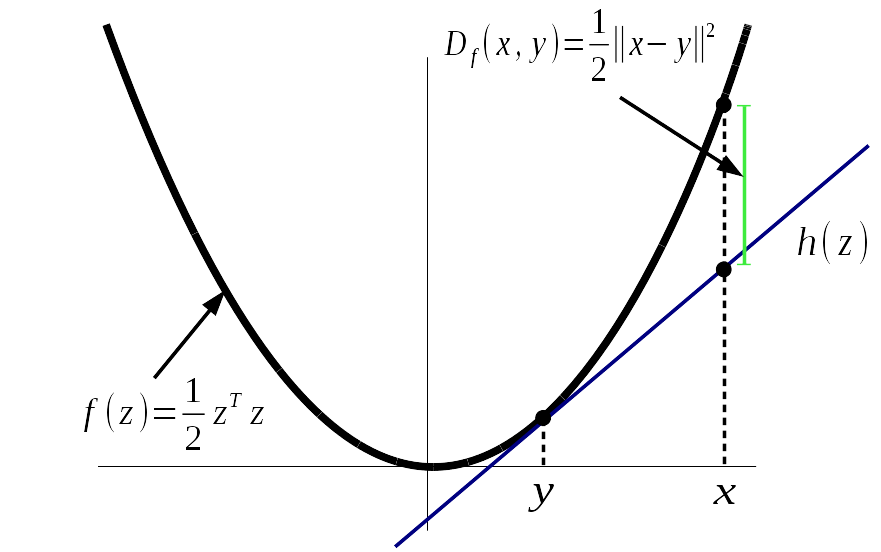
\includegraphics[width=0.6\columnwidth]{Figures/bregman_projection}
%\caption{Geometry of the Bregman divergence with the seed function $f(z)=\frac{1}{2}z^\intercal z$. $h(z)$ is a hyperplane tangent to $f(z)$ at $y$. While it accurately represent $f(y)$, it underestimate $f(x)$. The Bregman divergence measures how much the representation of $f(x)$ on $h(z)$ \emph{diverges} from $f(x)$ (in green).}
%\label{fig:bregman-projection}
%\end{figure}